% Options for packages loaded elsewhere
\PassOptionsToPackage{unicode}{hyperref}
\PassOptionsToPackage{hyphens}{url}
\PassOptionsToPackage{dvipsnames,svgnames,x11names}{xcolor}
%
\documentclass[
]{article}

\usepackage{amsmath,amssymb}
\usepackage{iftex}
\ifPDFTeX
  \usepackage[T1]{fontenc}
  \usepackage[utf8]{inputenc}
  \usepackage{textcomp} % provide euro and other symbols
\else % if luatex or xetex
  \usepackage{unicode-math}
  \defaultfontfeatures{Scale=MatchLowercase}
  \defaultfontfeatures[\rmfamily]{Ligatures=TeX,Scale=1}
\fi
\usepackage{lmodern}
\ifPDFTeX\else  
    % xetex/luatex font selection
\fi
% Use upquote if available, for straight quotes in verbatim environments
\IfFileExists{upquote.sty}{\usepackage{upquote}}{}
\IfFileExists{microtype.sty}{% use microtype if available
  \usepackage[]{microtype}
  \UseMicrotypeSet[protrusion]{basicmath} % disable protrusion for tt fonts
}{}
\makeatletter
\@ifundefined{KOMAClassName}{% if non-KOMA class
  \IfFileExists{parskip.sty}{%
    \usepackage{parskip}
  }{% else
    \setlength{\parindent}{0pt}
    \setlength{\parskip}{6pt plus 2pt minus 1pt}}
}{% if KOMA class
  \KOMAoptions{parskip=half}}
\makeatother
\usepackage{xcolor}
\setlength{\emergencystretch}{3em} % prevent overfull lines
\setcounter{secnumdepth}{5}
% Make \paragraph and \subparagraph free-standing
\makeatletter
\ifx\paragraph\undefined\else
  \let\oldparagraph\paragraph
  \renewcommand{\paragraph}{
    \@ifstar
      \xxxParagraphStar
      \xxxParagraphNoStar
  }
  \newcommand{\xxxParagraphStar}[1]{\oldparagraph*{#1}\mbox{}}
  \newcommand{\xxxParagraphNoStar}[1]{\oldparagraph{#1}\mbox{}}
\fi
\ifx\subparagraph\undefined\else
  \let\oldsubparagraph\subparagraph
  \renewcommand{\subparagraph}{
    \@ifstar
      \xxxSubParagraphStar
      \xxxSubParagraphNoStar
  }
  \newcommand{\xxxSubParagraphStar}[1]{\oldsubparagraph*{#1}\mbox{}}
  \newcommand{\xxxSubParagraphNoStar}[1]{\oldsubparagraph{#1}\mbox{}}
\fi
\makeatother

\usepackage{color}
\usepackage{fancyvrb}
\newcommand{\VerbBar}{|}
\newcommand{\VERB}{\Verb[commandchars=\\\{\}]}
\DefineVerbatimEnvironment{Highlighting}{Verbatim}{commandchars=\\\{\}}
% Add ',fontsize=\small' for more characters per line
\usepackage{framed}
\definecolor{shadecolor}{RGB}{241,243,245}
\newenvironment{Shaded}{\begin{snugshade}}{\end{snugshade}}
\newcommand{\AlertTok}[1]{\textcolor[rgb]{0.68,0.00,0.00}{#1}}
\newcommand{\AnnotationTok}[1]{\textcolor[rgb]{0.37,0.37,0.37}{#1}}
\newcommand{\AttributeTok}[1]{\textcolor[rgb]{0.40,0.45,0.13}{#1}}
\newcommand{\BaseNTok}[1]{\textcolor[rgb]{0.68,0.00,0.00}{#1}}
\newcommand{\BuiltInTok}[1]{\textcolor[rgb]{0.00,0.23,0.31}{#1}}
\newcommand{\CharTok}[1]{\textcolor[rgb]{0.13,0.47,0.30}{#1}}
\newcommand{\CommentTok}[1]{\textcolor[rgb]{0.37,0.37,0.37}{#1}}
\newcommand{\CommentVarTok}[1]{\textcolor[rgb]{0.37,0.37,0.37}{\textit{#1}}}
\newcommand{\ConstantTok}[1]{\textcolor[rgb]{0.56,0.35,0.01}{#1}}
\newcommand{\ControlFlowTok}[1]{\textcolor[rgb]{0.00,0.23,0.31}{\textbf{#1}}}
\newcommand{\DataTypeTok}[1]{\textcolor[rgb]{0.68,0.00,0.00}{#1}}
\newcommand{\DecValTok}[1]{\textcolor[rgb]{0.68,0.00,0.00}{#1}}
\newcommand{\DocumentationTok}[1]{\textcolor[rgb]{0.37,0.37,0.37}{\textit{#1}}}
\newcommand{\ErrorTok}[1]{\textcolor[rgb]{0.68,0.00,0.00}{#1}}
\newcommand{\ExtensionTok}[1]{\textcolor[rgb]{0.00,0.23,0.31}{#1}}
\newcommand{\FloatTok}[1]{\textcolor[rgb]{0.68,0.00,0.00}{#1}}
\newcommand{\FunctionTok}[1]{\textcolor[rgb]{0.28,0.35,0.67}{#1}}
\newcommand{\ImportTok}[1]{\textcolor[rgb]{0.00,0.46,0.62}{#1}}
\newcommand{\InformationTok}[1]{\textcolor[rgb]{0.37,0.37,0.37}{#1}}
\newcommand{\KeywordTok}[1]{\textcolor[rgb]{0.00,0.23,0.31}{\textbf{#1}}}
\newcommand{\NormalTok}[1]{\textcolor[rgb]{0.00,0.23,0.31}{#1}}
\newcommand{\OperatorTok}[1]{\textcolor[rgb]{0.37,0.37,0.37}{#1}}
\newcommand{\OtherTok}[1]{\textcolor[rgb]{0.00,0.23,0.31}{#1}}
\newcommand{\PreprocessorTok}[1]{\textcolor[rgb]{0.68,0.00,0.00}{#1}}
\newcommand{\RegionMarkerTok}[1]{\textcolor[rgb]{0.00,0.23,0.31}{#1}}
\newcommand{\SpecialCharTok}[1]{\textcolor[rgb]{0.37,0.37,0.37}{#1}}
\newcommand{\SpecialStringTok}[1]{\textcolor[rgb]{0.13,0.47,0.30}{#1}}
\newcommand{\StringTok}[1]{\textcolor[rgb]{0.13,0.47,0.30}{#1}}
\newcommand{\VariableTok}[1]{\textcolor[rgb]{0.07,0.07,0.07}{#1}}
\newcommand{\VerbatimStringTok}[1]{\textcolor[rgb]{0.13,0.47,0.30}{#1}}
\newcommand{\WarningTok}[1]{\textcolor[rgb]{0.37,0.37,0.37}{\textit{#1}}}

\providecommand{\tightlist}{%
  \setlength{\itemsep}{0pt}\setlength{\parskip}{0pt}}\usepackage{longtable,booktabs,array}
\usepackage{calc} % for calculating minipage widths
% Correct order of tables after \paragraph or \subparagraph
\usepackage{etoolbox}
\makeatletter
\patchcmd\longtable{\par}{\if@noskipsec\mbox{}\fi\par}{}{}
\makeatother
% Allow footnotes in longtable head/foot
\IfFileExists{footnotehyper.sty}{\usepackage{footnotehyper}}{\usepackage{footnote}}
\makesavenoteenv{longtable}
\usepackage{graphicx}
\makeatletter
\def\maxwidth{\ifdim\Gin@nat@width>\linewidth\linewidth\else\Gin@nat@width\fi}
\def\maxheight{\ifdim\Gin@nat@height>\textheight\textheight\else\Gin@nat@height\fi}
\makeatother
% Scale images if necessary, so that they will not overflow the page
% margins by default, and it is still possible to overwrite the defaults
% using explicit options in \includegraphics[width, height, ...]{}
\setkeys{Gin}{width=\maxwidth,height=\maxheight,keepaspectratio}
% Set default figure placement to htbp
\makeatletter
\def\fps@figure{htbp}
\makeatother
% definitions for citeproc citations
\NewDocumentCommand\citeproctext{}{}
\NewDocumentCommand\citeproc{mm}{%
  \begingroup\def\citeproctext{#2}\cite{#1}\endgroup}
\makeatletter
 % allow citations to break across lines
 \let\@cite@ofmt\@firstofone
 % avoid brackets around text for \cite:
 \def\@biblabel#1{}
 \def\@cite#1#2{{#1\if@tempswa , #2\fi}}
\makeatother
\newlength{\cslhangindent}
\setlength{\cslhangindent}{1.5em}
\newlength{\csllabelwidth}
\setlength{\csllabelwidth}{3em}
\newenvironment{CSLReferences}[2] % #1 hanging-indent, #2 entry-spacing
 {\begin{list}{}{%
  \setlength{\itemindent}{0pt}
  \setlength{\leftmargin}{0pt}
  \setlength{\parsep}{0pt}
  % turn on hanging indent if param 1 is 1
  \ifodd #1
   \setlength{\leftmargin}{\cslhangindent}
   \setlength{\itemindent}{-1\cslhangindent}
  \fi
  % set entry spacing
  \setlength{\itemsep}{#2\baselineskip}}}
 {\end{list}}
\usepackage{calc}
\newcommand{\CSLBlock}[1]{\hfill\break\parbox[t]{\linewidth}{\strut\ignorespaces#1\strut}}
\newcommand{\CSLLeftMargin}[1]{\parbox[t]{\csllabelwidth}{\strut#1\strut}}
\newcommand{\CSLRightInline}[1]{\parbox[t]{\linewidth - \csllabelwidth}{\strut#1\strut}}
\newcommand{\CSLIndent}[1]{\hspace{\cslhangindent}#1}

\makeatletter
\@ifpackageloaded{caption}{}{\usepackage{caption}}
\AtBeginDocument{%
\ifdefined\contentsname
  \renewcommand*\contentsname{Table of contents}
\else
  \newcommand\contentsname{Table of contents}
\fi
\ifdefined\listfigurename
  \renewcommand*\listfigurename{List of Figures}
\else
  \newcommand\listfigurename{List of Figures}
\fi
\ifdefined\listtablename
  \renewcommand*\listtablename{List of Tables}
\else
  \newcommand\listtablename{List of Tables}
\fi
\ifdefined\figurename
  \renewcommand*\figurename{Figure}
\else
  \newcommand\figurename{Figure}
\fi
\ifdefined\tablename
  \renewcommand*\tablename{Table}
\else
  \newcommand\tablename{Table}
\fi
}
\@ifpackageloaded{float}{}{\usepackage{float}}
\floatstyle{ruled}
\@ifundefined{c@chapter}{\newfloat{codelisting}{h}{lop}}{\newfloat{codelisting}{h}{lop}[chapter]}
\floatname{codelisting}{Listing}
\newcommand*\listoflistings{\listof{codelisting}{List of Listings}}
\makeatother
\makeatletter
\makeatother
\makeatletter
\@ifpackageloaded{caption}{}{\usepackage{caption}}
\@ifpackageloaded{subcaption}{}{\usepackage{subcaption}}
\makeatother

\ifLuaTeX
  \usepackage{selnolig}  % disable illegal ligatures
\fi
\usepackage{bookmark}

\IfFileExists{xurl.sty}{\usepackage{xurl}}{} % add URL line breaks if available
\urlstyle{same} % disable monospaced font for URLs
\hypersetup{
  pdftitle={Exploratory Analysis of World Development Indicators},
  pdfauthor={Tomas Hossain-Aguilar},
  colorlinks=true,
  linkcolor={blue},
  filecolor={Maroon},
  citecolor={Blue},
  urlcolor={Blue},
  pdfcreator={LaTeX via pandoc}}


\title{Exploratory Analysis of World Development Indicators}
\author{Tomas Hossain-Aguilar}
\date{2024-10-07}

\begin{document}
\maketitle

\renewcommand*\contentsname{Table of contents}
{
\hypersetup{linkcolor=}
\setcounter{tocdepth}{3}
\tableofcontents
}

\section{Exploratory Data Analysis of Nation GDP per capita,
Life-Expectancies and Education
Expenditure}\label{exploratory-data-analysis-of-nation-gdp-per-capita-life-expectancies-and-education-expenditure}

This report serves to visualize and detail distributions of global GDP
per capitas, Life-Expectancies, and Education Expenditure.

The relationship between GDP per capita and Life-Expectancy will be
explored, as well as nation's expenditure on education as a proportion
of total GDP.

\subsection{GDP per capita}\label{gdp-per-capita}

The \textbf{GDP per capita} for the 203 countries in the dataset
exhibits a wide range, reflecting significant disparities in economic
prosperity across the world. The mean GDP per capita is approximately
\textbf{\$20,345.71}, with a standard deviation of \textbf{\$31,308.94},
indicating substantial variability among countries.

\begin{figure}

\centering{

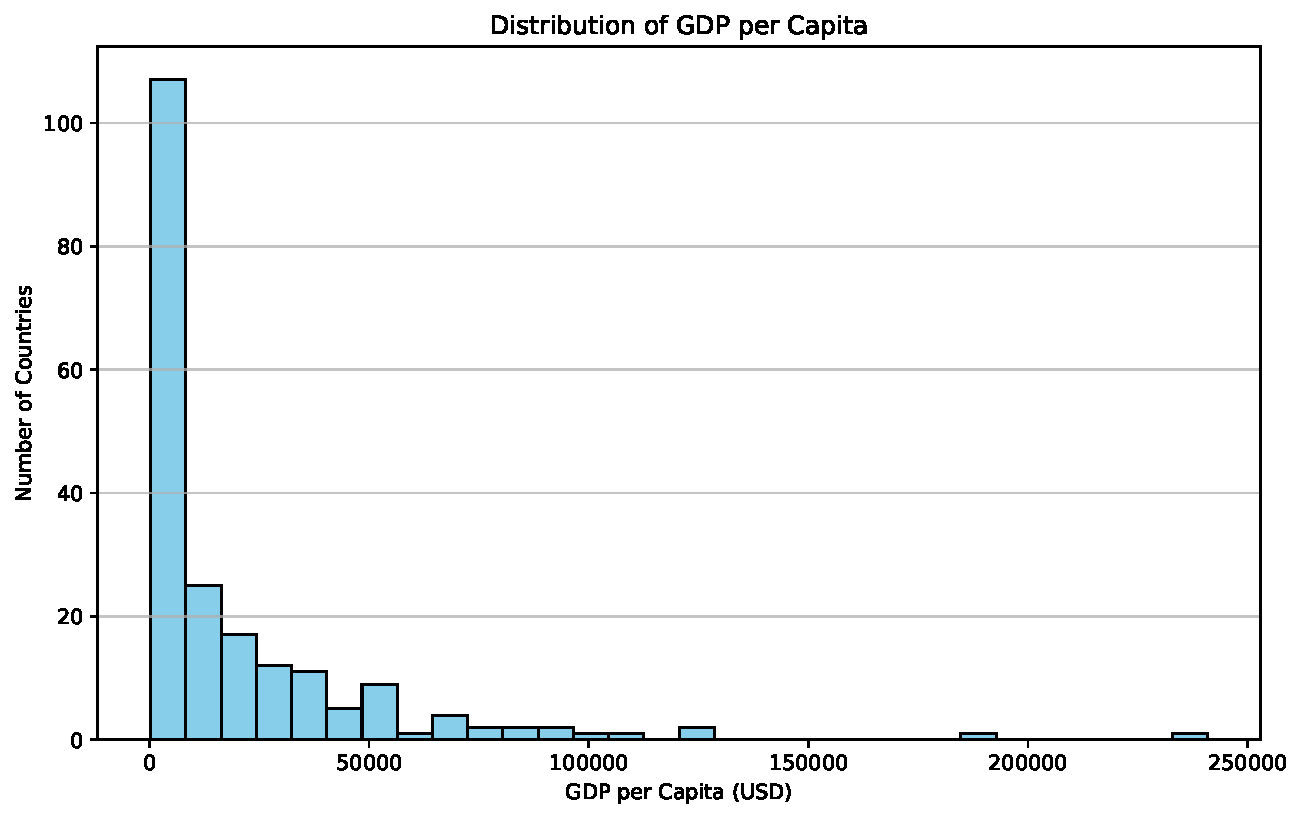
\includegraphics{report_files/figure-pdf/fig-gdp-histogram-output-1.pdf}

}

\caption{\label{fig-gdp-histogram}Figure 3: Distribution of GDP per
Capita (2022). Source: World Development Indicators.}

\end{figure}%

More Key Statistics:

\begin{itemize}
\tightlist
\item
  \textbf{Minimum GDP per Capita:} \$259.03
\item
  \textbf{Maximum GDP per Capita:} \$240,862.18
\item
  \textbf{Median (50th percentile):} \$7,587.59
\item
  \textbf{25th percentile:} \$2,570.56
\item
  \textbf{75th percentile:} \$25,982.63
\end{itemize}

The median GDP per capita is significantly lower than the mean,
suggesting a right-skewed distribution where a small number of countries
have very high GDP per capita values, elevating the average. We observe
this skew in Figure~\ref{fig-gdp-histogram}, above. The majority of
countries have GDP per capita values clustered between the 25th and 75th
percentiles (\$2,570.56 to \$25,982.63).

\phantomsection\label{gdp-summary-stats}
\begin{Shaded}
\begin{Highlighting}[]
\NormalTok{gdp\_per\_capita\_stats }\OperatorTok{=}\NormalTok{ data[}\StringTok{\textquotesingle{}gdp\_per\_capita\textquotesingle{}}\NormalTok{].describe()}
\BuiltInTok{print}\NormalTok{(}\StringTok{"GDP per Capita Statistics:"}\NormalTok{)}
\BuiltInTok{print}\NormalTok{(gdp\_per\_capita\_stats)}
\end{Highlighting}
\end{Shaded}

\begin{verbatim}
GDP per Capita Statistics:
count       203.000000
mean      20345.707649
std       31308.942225
min         259.025031
25%        2570.563284
50%        7587.588173
75%       25982.630050
max      240862.182448
Name: gdp_per_capita, dtype: float64
\end{verbatim}

\subsection{Life Expectancy}\label{life-expectancy}

The \textbf{Life Expectancy} data for 209 countries shows a global
average of \textbf{72.42 years}, with a standard deviation of
\textbf{7.71 years}, indicating moderate variation across countries.

\begin{figure}

\centering{

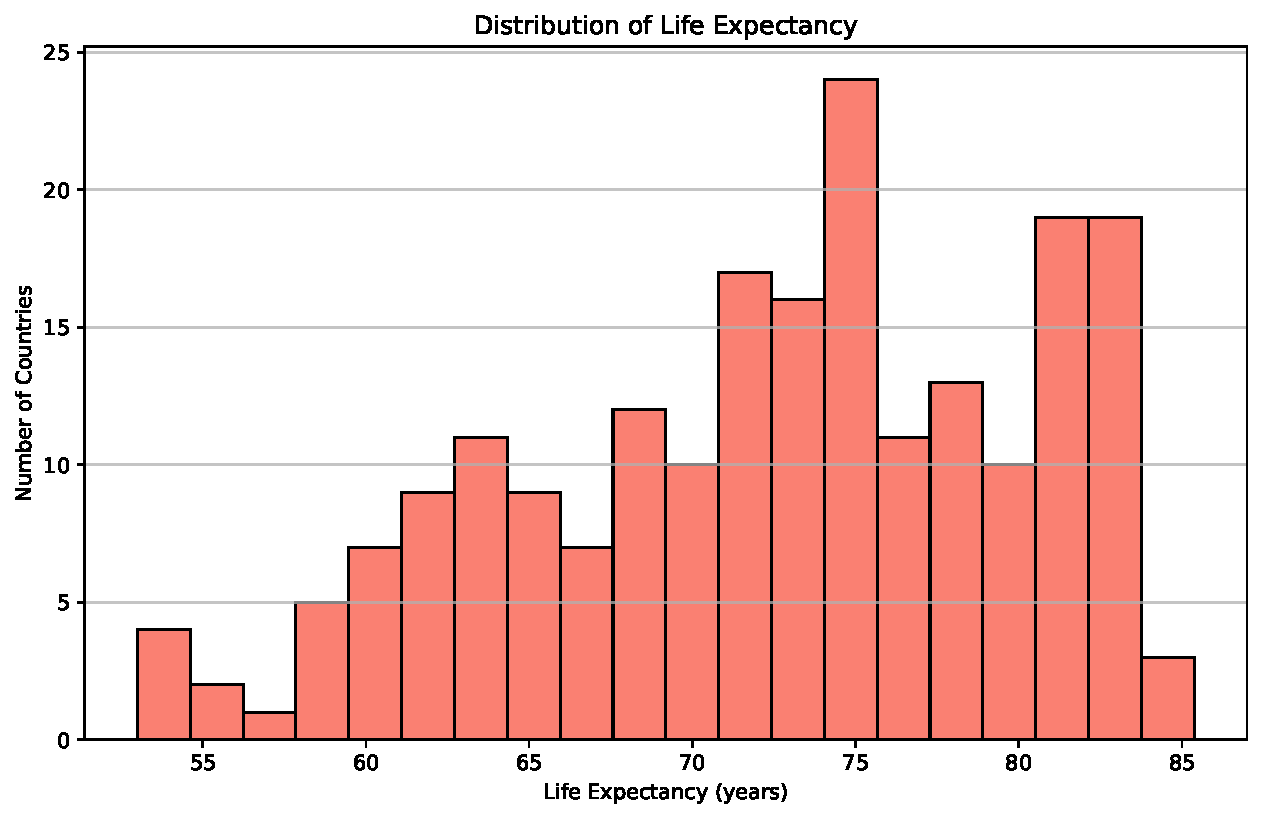
\includegraphics{report_files/figure-pdf/fig-life-expectancy-histogram-output-1.pdf}

}

\caption{\label{fig-life-expectancy-histogram}Figure 4: Distribution of
Life Expectancy (2022). Source: World Development Indicators.}

\end{figure}%

More Key Statistics:

\begin{itemize}
\tightlist
\item
  \textbf{Minimum Life Expectancy:} 52.997 years
\item
  \textbf{Maximum Life Expectancy:} 85.377 years
\item
  \textbf{Median (50th percentile):} 73.51 years
\item
  \textbf{25th percentile:} 66.78 years
\item
  \textbf{75th percentile:} 78.475 years
\end{itemize}

The median life expectancy is slightly higher than the mean, suggesting
a relatively symmetrical distribution, which we can observe in the
figure above, Figure~\ref{fig-life-expectancy-histogram}. The
interquartile range (66.78 to 78.475 years) captures the middle 50\% of
countries, highlighting that most countries have life expectancies
within this range. The gap between the minimum and maximum values
underscores significant differences in health outcomes and living
conditions worldwide.

The scatter plot in Figure Figure~\ref{fig-gdp-life} presents the
relationship between GDP per capita and life expectancy across various
countries in 2022. An analysis of this graph reveals several important
insights. Observe a positive correlation between GDP per capita and life
expectancy, as well as `diminishing returns' as GDP per capita
increases. This indicates that GDP per capita is less related to life
expectancy for countries as GDP per capita increases.

\begin{figure}

\centering{

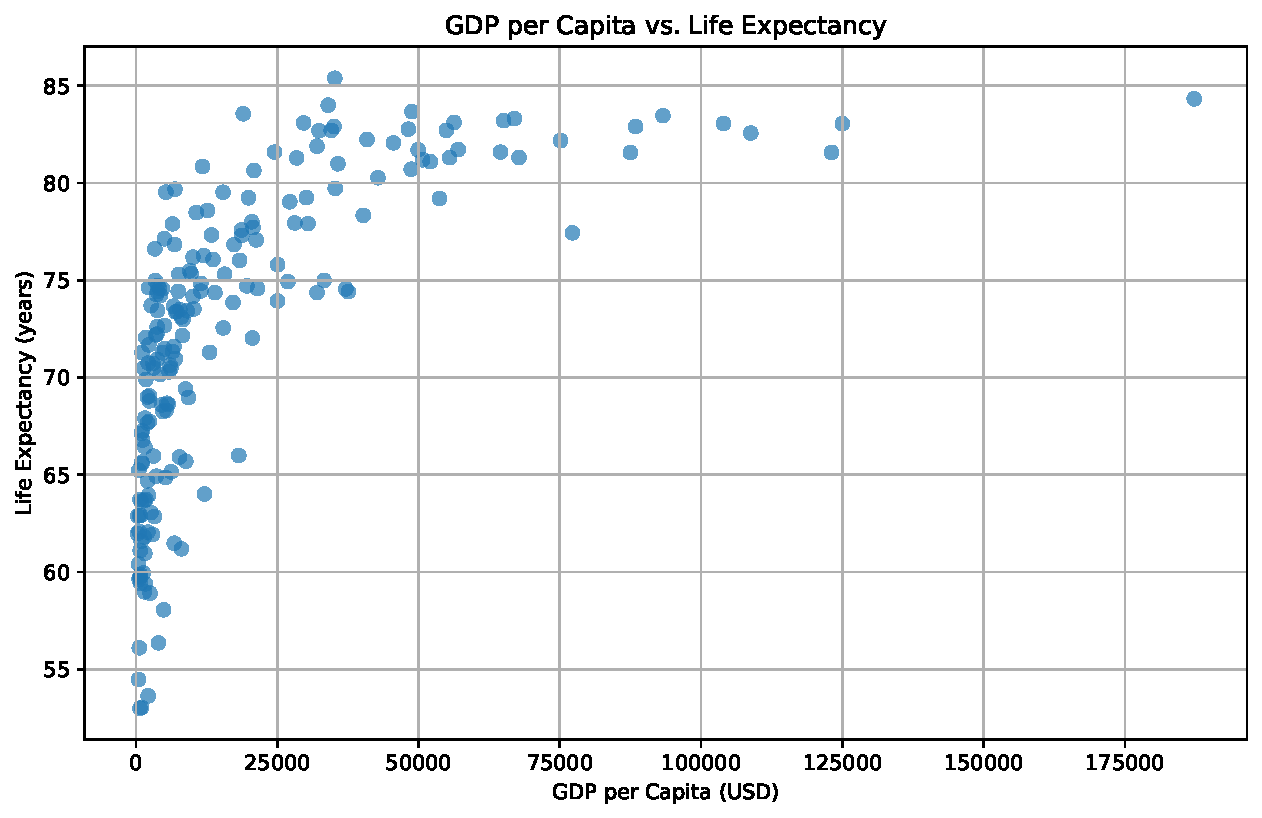
\includegraphics{report_files/figure-pdf/fig-gdp-life-output-1.pdf}

}

\caption{\label{fig-gdp-life}Figure 1: GDP per Capita vs.~Life
Expectancy (2022). Source: World Development Indicators.}

\end{figure}%

\phantomsection\label{life-expectancy-summary-stats}
\begin{Shaded}
\begin{Highlighting}[]
\NormalTok{life\_expectancy\_stats }\OperatorTok{=}\NormalTok{ data[}\StringTok{\textquotesingle{}life\_expectancy\textquotesingle{}}\NormalTok{].describe()}
\BuiltInTok{print}\NormalTok{(}\StringTok{"}\CharTok{\textbackslash{}n}\StringTok{Life Expectancy Statistics:"}\NormalTok{)}
\BuiltInTok{print}\NormalTok{(life\_expectancy\_stats)}
\end{Highlighting}
\end{Shaded}

\begin{verbatim}

Life Expectancy Statistics:
count    209.000000
mean      72.416519
std        7.713322
min       52.997000
25%       66.782000
50%       73.514634
75%       78.475000
max       85.377000
Name: life_expectancy, dtype: float64
\end{verbatim}

\subsection{Education Expenditure (\% of
GDP)}\label{education-expenditure-of-gdp}

For Education Expenditure as a percentage of GDP, data is available for
105 countries. The mean expenditure is 4.23\% of GDP, with a standard
deviation of 2.07\%, reflecting variability in national investment in
education.

\begin{figure}

\centering{

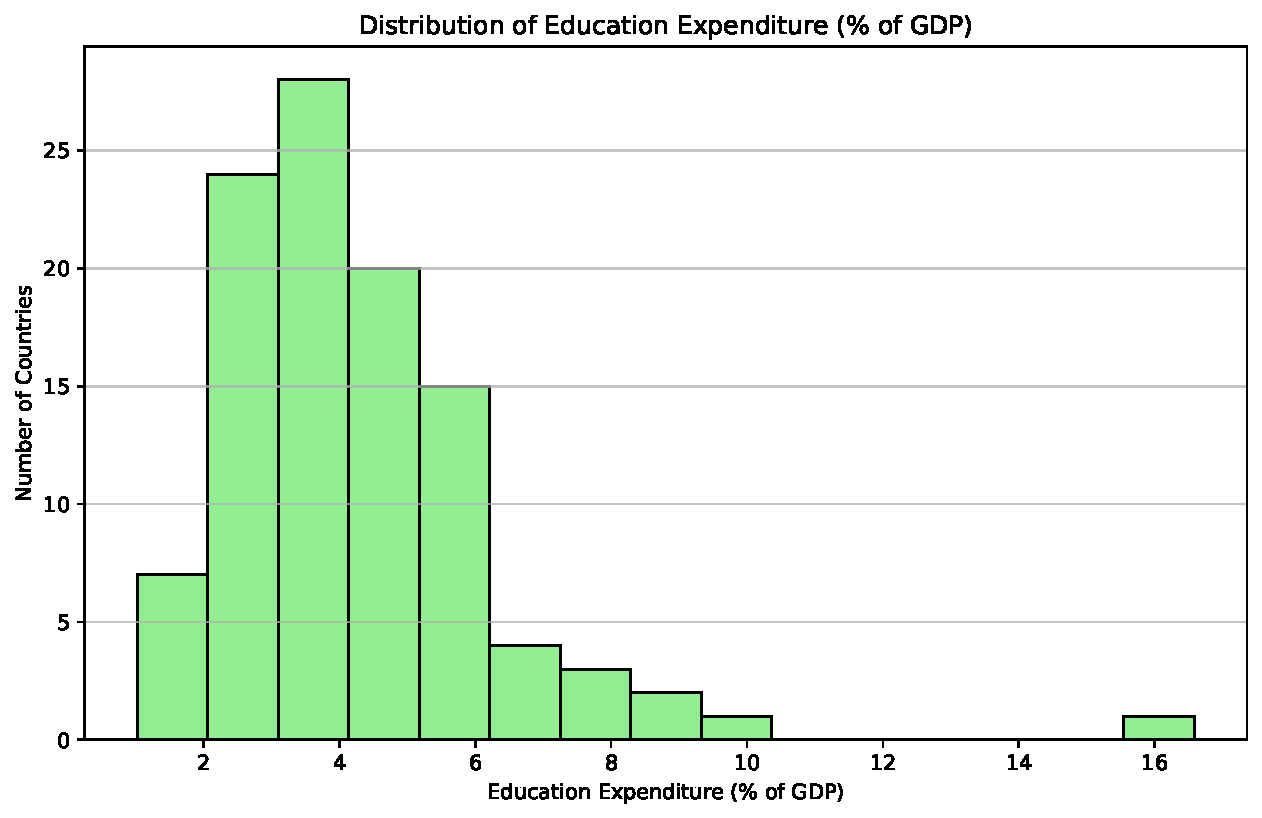
\includegraphics{report_files/figure-pdf/fig-education-expenditure-histogram-output-1.pdf}

}

\caption{\label{fig-education-expenditure-histogram}Figure 5:
Distribution of Education Expenditure (\% of GDP) (2022). Source: World
Development Indicators.}

\end{figure}%

More Key Statistics:

\begin{itemize}
\tightlist
\item
  Minimum Education Expenditure: 1.027\%
\item
  Maximum Education Expenditure: 16.582\%
\item
  Median (50th percentile): 3.887\%
\item
  25th percentile: 2.898\%
\item
  75th percentile: 5.156\%
\end{itemize}

The median expenditure is slightly below the mean, indicating a slight
left-skew in the distribution, which we can again observe above, in
Figure~\ref{fig-education-expenditure-histogram}. The majority of
countries spend between approximately 2.90\% and 5.16\% of their GDP on
education. The maximum value of 16.58\% suggests that some countries
prioritize education significantly more than others relative to their
economic output.

\begin{figure}

\centering{

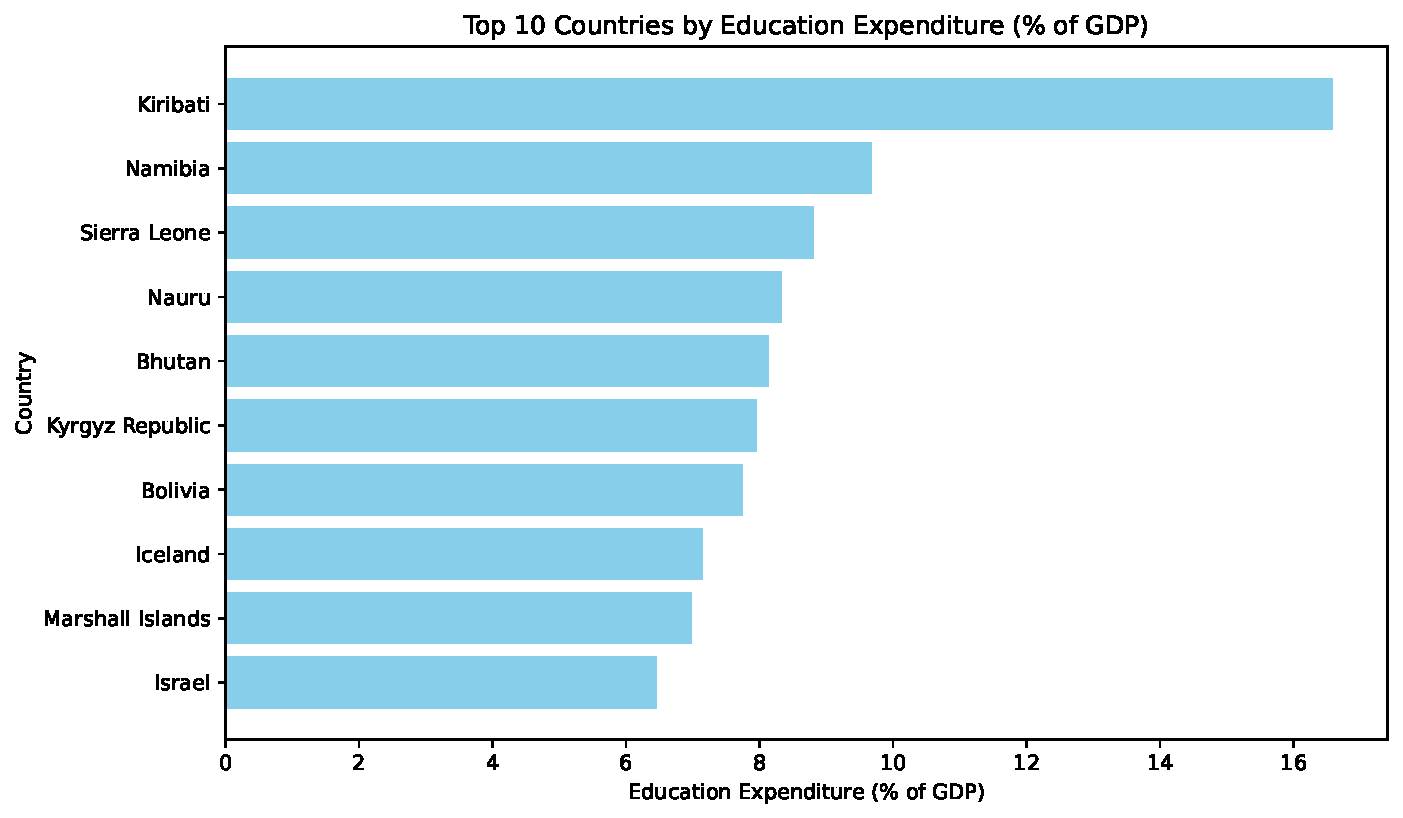
\includegraphics{report_files/figure-pdf/fig-education-expenditure-output-1.pdf}

}

\caption{\label{fig-education-expenditure}Figure 2: Top 10 Countries by
Education Expenditure (\% of GDP) (2022). Source: World Development
Indicators.}

\end{figure}%

\phantomsection\label{education-expenditure-summary-stats}
\begin{Shaded}
\begin{Highlighting}[]
\NormalTok{education\_expenditure\_stats }\OperatorTok{=}\NormalTok{ data[}\StringTok{\textquotesingle{}education\_expenditure\_gdp\_share\textquotesingle{}}\NormalTok{].describe()}
\BuiltInTok{print}\NormalTok{(}\StringTok{"}\CharTok{\textbackslash{}n}\StringTok{Education Expenditure (}\SpecialCharTok{\% o}\StringTok{f GDP) Statistics:"}\NormalTok{)}
\BuiltInTok{print}\NormalTok{(education\_expenditure\_stats)}
\end{Highlighting}
\end{Shaded}

\begin{verbatim}

Education Expenditure (% of GDP) Statistics:
count    105.000000
mean       4.226215
std        2.069486
min        1.027000
25%        2.898000
50%        3.887000
75%        5.156000
max       16.582462
Name: education_expenditure_gdp_share, dtype: float64
\end{verbatim}

\section{Takeaways}\label{takeaways}

\subsection{Revisiting Summary
Statistics}\label{revisiting-summary-statistics}

\begin{table}

\caption{\label{tbl-key-stats}Table 1: Key Statistics of Selected
Indicators.}

\centering{

\begin{verbatim}
       gdp_per_capita  life_expectancy  education_expenditure_gdp_share
count          203.00           209.00                           105.00
mean         20345.71            72.42                             4.23
std          31308.94             7.71                             2.07
min            259.03            53.00                             1.03
25%           2570.56            66.78                             2.90
50%           7587.59            73.51                             3.89
75%          25982.63            78.47                             5.16
max         240862.18            85.38                            16.58
\end{verbatim}

}

\end{table}%

\subsection{McKinsey's Analysis ``Pixel's of Progress: Chapter
3''}\label{mckinseys-analysis-pixels-of-progress-chapter-3}

Our analysis of the relationship between \textbf{GDP per capita} and
\textbf{life expectancy} in Figure Figure~\ref{fig-gdp-life} reveals a
positive correlation, indicating that higher economic prosperity
generally leads to better health outcomes. However, we also observed
diminishing returns at higher GDP levels and significant variability
among countries with similar economic standings. This suggests that
factors beyond mere economic wealth---such as healthcare infrastructure,
education quality, and social policies---play crucial roles in
determining life expectancy.

McKinsey Global Institute's ``Pixels of Progress: Chapter 3'' McKinsey
Global Institute (2023) echoes these findings by exploring how
advancements in various sectors contribute to human development beyond
traditional economic metrics. The article emphasizes that while economic
growth is essential, it is not sufficient on its own to ensure improved
life expectancy and overall well-being. Investments in
\textbf{healthcare access}, \textbf{education}, and
\textbf{technological innovation} are highlighted as critical drivers of
progress.

\phantomsection\label{refs}
\begin{CSLReferences}{1}{0}
\bibitem[\citeproctext]{ref-mckinsey2023pixels}
McKinsey Global Institute. 2023. {``Pixels of Progress: Chapter 3.''}
\url{https://www.mckinsey.com/mgi/our-research/pixels-of-progress-chapter-3}.

\end{CSLReferences}




\end{document}
